\documentclass[a4paper]{article}

%use the english line for english reports
%usepackage[english]{babel}
\usepackage[portuguese]{babel}
\usepackage[utf8]{inputenc}
\usepackage{indentfirst}
\usepackage{graphicx}
\usepackage{verbatim}
\usepackage{listings}


\begin{document}

\setlength{\textwidth}{16cm}
\setlength{\textheight}{22cm}

\title{\Huge\textbf{Xadrersi}\linebreak\linebreak\linebreak
\Large\textbf{Relatório Intercalar}\linebreak\linebreak
\linebreak\linebreak

\includegraphics[scale=0.1]{feup-logo.png}\linebreak\linebreak
\linebreak\linebreak
\Large{Mestrado Integrado em Engenharia Informática e Computação} \linebreak\linebreak
\Large{Programação em Lógica}\linebreak
}

\author{\textbf{Grupo Xadrersi\_1:}\\
António Cunha Seco Fernandes de Almeida - 201505836 \\
João Paulo Madureira Damas - 201504088 \\
\linebreak\linebreak \\
 \\ Faculdade de Engenharia da Universidade do Porto \\ Rua Roberto Frias, s\/n, 4200-465 Porto, Portugal \linebreak\linebreak\linebreak
\linebreak\linebreak\vspace{1cm}}

\maketitle
\thispagestyle{empty}

%************************************************************************************************
%************************************************************************************************

\newpage

%Todas as figuras devem ser referidas no texto. %\ref{fig:codigoFigura}
%
%%Exemplo de código para inserção de figuras
%%\begin{figure}[h!]
%%\begin{center}
%%escolher entre uma das seguintes três linhas:
%%\includegraphics[height=20cm,width=15cm]{path relativo da imagem}
%%\includegraphics[scale=0.5]{path relativo da imagem}
%%\includegraphics{path relativo da imagem}
%%\caption{legenda da figura}
%%\label{fig:codigoFigura}
%%\end{center}
%%\end{figure}
%
%
%\textit{Para escrever em itálico}
%\textbf{Para escrever em negrito}
%Para escrever em letra normal
%``Para escrever texto entre aspas''
%
%Para fazer parágrafo, deixar uma linha em branco.
%
%Como fazer bullet points:
%\begin{itemize}
	%\item Item1
	%\item Item2
%\end{itemize}
%
%Como enumerar itens:
%\begin{enumerate}
	%\item Item 1
	%\item Item 2
%\end{enumerate}
%
%\begin{quote}``Isto é uma citação''\end{quote}


%%%%%%%%%%%%%%%%%%%%%%%%%%
\section{O Jogo Xadrersi}

\textbf{Origens}\linebreak

Xadrersi é um jogo de tabuleiro para duas pessoas criado por Andi Lewicki, em 2003. Como o nome sugere, surge de uma combinação entre os conhecidos jogos de tabuleiro Xadrez e Reversi.\newline

\textbf{Regras}\newline

O jogo é disputado num tradicional tabuleiro 8x8, inicialmente vazio. A seu dispor, cada jogador possui as peças de que disporia se estivesse numa partida de Xadrez, exceto peões.
Por outras palavras, cada jogador possui um rei, uma rainha, dois cavalos, dois bispos e duas torres.\newline

Os jogadores vão colocando as suas peças no tabuleiro, uma a uma, alternadamente, até todas as peças estarem em jogo.
Após colocada, uma peça não pode ser movida nem retirada (capturada).
No entanto, ataca outras posições do tabuleiro segundo as regras de Xadrez (o rei ataca as posições adjacentes, o bispo diagonalmente, o cavalo em 'L', etc).
Não se aplicam regras de cheque nem afastamento obrigatório entre reis, logo um rei pode ser colocado numa posição onde ficaria em cheque e os reis podem ficar em posições adjacentes. Os bispos devem ficar em posições de cores opostas, como no Xadrez.\newline

De uma maneira geral, cada jogada é válida se e só se a peça colocada estiver a ser atacada por pelo menos uma peça adversária. A primeira exceção a esta regra é a primeira jogada, em que não há peças no tabuleiro. O jogador com as peças brancas começa e a primeira peça jogada é obrigatoriamente o rei, podendo ser colocado em qualquer posição.
As figuras \ref{fig:fig1}, \ref{fig:fig2} e \ref{fig:fig3} ilustram uma sequência de jogadas válidas (com as hipóteses em cada turno destacadas) a partir da posição inicial.

\begin{small}
\begin{figure}[!htb]
\minipage{0.2\textwidth}
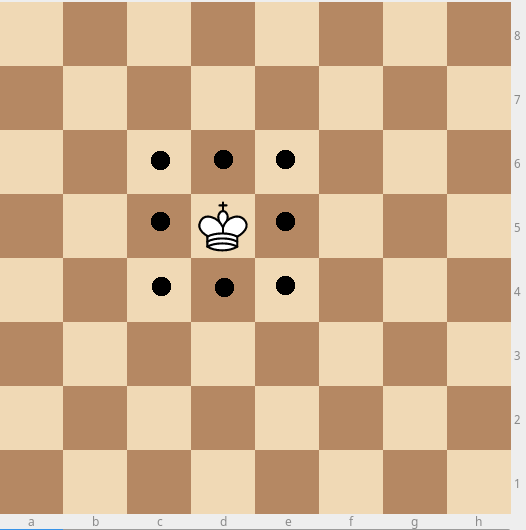
\includegraphics[scale=0.2]{board1.png}
\caption{\textit{Após a primeira jogada, uma peça preta tem de ser colocada adjacentemente ao rei branco de modo a poder ser atacada por este, constituindo uma jogada válida}}
\label{fig:fig1}
\endminipage\hfill
\minipage{0.2\textwidth}
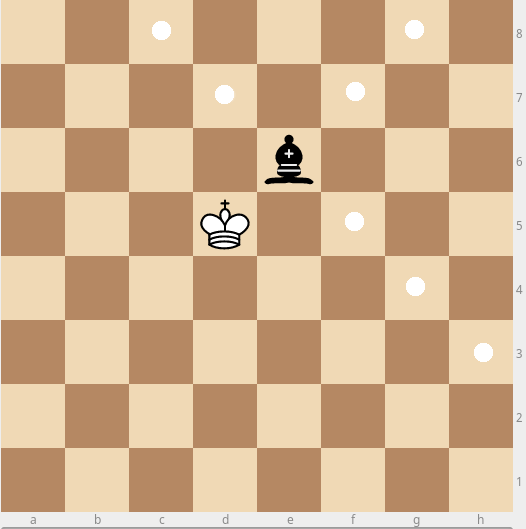
\includegraphics[scale=0.2]{board2.png}
\caption{\textit{Agora, tendo o jogador de peças pretas jogado um bispo, o jogador de peças brancas deve colocar uma peça que intersete o mesmo segundo uma das suas diagonais livres}}
\label{fig:fig2}
\endminipage\hfill
\minipage{0.2\textwidth}
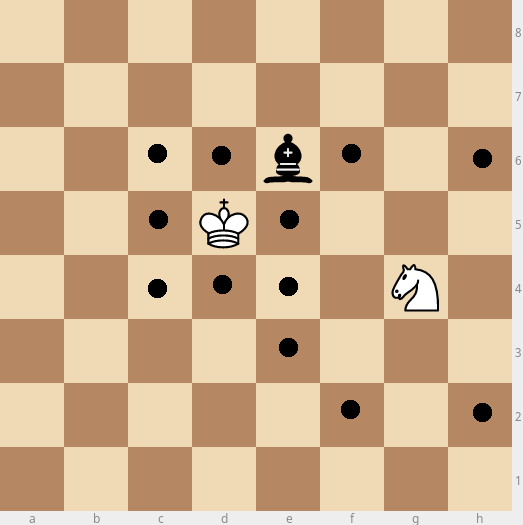
\includegraphics[scale=0.2]{board3.png}
\caption{\textit{Neste caso, tendo já mais do que uma peça branca em jogo, o jogador de peças pretas apenas precisa de se certificar que a peça que colocar é atacada por pelo menos uma peça branca}}
\label{fig:fig3}
\endminipage
\end{figure}
\end{small}

Existe ainda outro caso excecional. Caso seja impossível colocar uma peça de tal modo que seja atacada por uma peça adversária, o jogador pode colocar a peça em qualquer posição livre no tabuleiro. Na figura \ref{fig:fig4} demonstra-se esta situação através de um caso simples.

\begin{figure}[h!]
\begin{center}
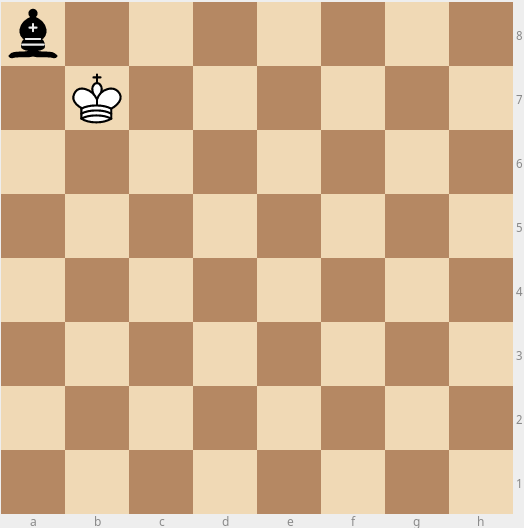
\includegraphics[scale=0.25]{board4.png}
\caption{\textit{Após a jogada inicial do rei, o bispo foi colocado em A8, adjacente ao rei e por isso válido. No entanto, a sua única diagonal está bloqueada e por isso nenhuma posição livre é atacada pelo mesmo. Nesta situação, aplica-se a exceção e a próxima peça branca pode ser colocada em qualquer posição livre.}}
\label{fig:fig4}
\end{center}
\end{figure}

Para além da obrigatoriedade do rei branco ser a primeira peça jogada, existem ainda duas regras adicionais a assinalar para tentar garantir o equilíbrio do jogo:
\begin{itemize}
    \item O rei preto é sempre a última peça a ser colocada no tabuleiro
    \item Quando um jogador coloca em jogo a sua rainha, o outro é obrigado, no turno seguinte, a colocar também a sua rainha em jogo
\end{itemize}

\textbf{Objetivo}\newline

O objetivo é conseguir o maior número de pontos quando o jogo terminar, ou seja, quando todas as peças forem colocadas no tabuleiro.
O número de pontos de um jogador corresponde ao número total de casas que as suas peças atacam.
Caso várias peças ataquem a mesma casa, esta é contabilizada uma vez por cada peça que a ataca.
Existe, por isso, a possibilidade de empate.

%%%%%%%%%%%%%%%%%%%%%%%%%%
\section{Representação do Estado do Jogo}

De forma a sistematizar uma relação entre a representação interna das pecas de jogo com a visualização das mesmas na consola, foi definida uma convenção. Os caracteres apresentados no ecrã baseam-se na nomenclatura em Inglês das peças de Xadrez, distinguindo-se as cores das mesmas através da utilização de maiúsculas ou minúsculas.

\begin{small}
\minipage{0.3\textwidth}

\large Peças Brancas
\begin{center}
  \begin{tabular}{ l | c | r }
    Rei & 1 & 'K' \\ \hline
    Rainha & 2 & 'Q' \\ \hline
    Bispo & 3 & 'B' \\ \hline
    Cavalo & 4 & 'H' \\ \hline
    Torre & 5 & 'R \\ 
  \end{tabular}
\end{center}

\endminipage\hfill
\minipage{0.3\textwidth}

\large Peças Pretas
\begin{center}
  \begin{tabular}{ l | c | r }
    Rei & 6 & 'k' \\ \hline
    Rainha & 7 & 'q' \\ \hline
    Bispo & 8 & 'b' \\ \hline
    Cavalo & 9 & 'h' \\ \hline
    Torre & 10 & 'r' \\ 
  \end{tabular}
\end{center}

\endminipage
\end{small} \newline\newline

Por último, uma casa vazia é internalmente representada como 0 e visualizada na consola como um espaço vazio. \newline

\large Estado Inicial de Jogo
\begin{center}
\begin{tabular}{c}
\begin{lstlisting}
[[0, 0, 0, 0, 0, 0, 0, 0],
[0, 0, 0, 0, 0, 0, 0, 0],
[0, 0, 0, 0, 0, 0, 0, 0],
[0, 0, 0, 0, 0, 0, 0, 0],
[0, 0, 0, 0, 0, 0, 0, 0],
[0, 0, 0, 0, 0, 0, 0, 0],
[0, 0, 0, 0, 0, 0, 0, 0],
[0, 0, 0, 0, 0, 0, 0, 0]]
\end{lstlisting}
\end{tabular}
\end{center}


\large Possível Estado Intermédio
\begin{center}
\begin{tabular}{c}
\begin{lstlisting}
[[0, 0, 0, 0, 0, 0, 0, 0],
[0, 0, 0, 0, 0, 0, 0, 0],
[0, 0, 0, 0, 8, 0, 0, 0],
[0, 0, 0, 1, 0, 0, 0, 0],
[0, 0, 0, 0, 0, 0, 4, 0],
[0, 0, 0, 0, 10, 0, 0, 0],
[0, 0, 0, 0, 0, 0, 0, 0],
[0, 0, 0, 0, 0, 0, 0, 0]]
\end{lstlisting}
\end{tabular}
\end{center}


%%%%%%%%%%%%%%%%%%%%%%%%%%
\section{Visualização do Tabuleiro}

Em modo de texto, serão utilizados os predicados seguintes para produzir uma representação dos estados de jogo. Bocados de código estão omitidos com reticências - '(...)' - por se tratarem de repetições de carateres ou padrões de caracteres.\linebreak

\begin{lstlisting}[language=Prolog]
getPieceDisplay(0, ' ').

%white pieces
getPieceDisplay(1, 'K').
getPieceDisplay(2, 'Q'). 
getPieceDisplay(3, 'B'). 
getPieceDisplay(4, 'H'). 
getPieceDisplay(5, 'R').

%black pieces
getPieceDisplay(6, 'k'). 
getPieceDisplay(7, 'q').
getPieceDisplay(8, 'b'). 
getPieceDisplay(9, 'h').
getPieceDisplay(10, 'r').

displayBoard( Board ) :-
	displayBoardHeader,
	N is 1, displayBoardTail(Board, N),
	displayBottom.

displayBoardTail([], 9).

displayBoardTail( [ Line | T ], N ):-
	write('|       |    (...)   |       |'), nl,
	write('------ (...) -------'), nl,
	write('|       |    (...)   |       |'), nl,
	displayLine(Line, N), nl,
	N1 is N+1,
	displayBoardTail(T, N1).

displayLine([], N):- 
	write('|  '), displayNumber(N).

displayLine( [ CurrentPiece | T ] , N ):-
	write('|   '),
	getPieceDisplay(CurrentPiece, PieceDisplay),
	write(PieceDisplay),
	write('   '),
	displayLine(T, N).

displayBoardHeader:- 
	nl,
	write('     a      b (...)  g       h '), nl.

displayBottom:-
	write('|       |    (...)   |       |'), nl,
	write('------ (...) -------'), nl.

displayNumber(N) :- write(N), !.
\end{lstlisting}

Os exemplos de estados de jogo apresentados na secção 2 são representados da seguinte forma:

\begin{small}
\begin{figure}[!htb]
\minipage{0.3\textwidth}
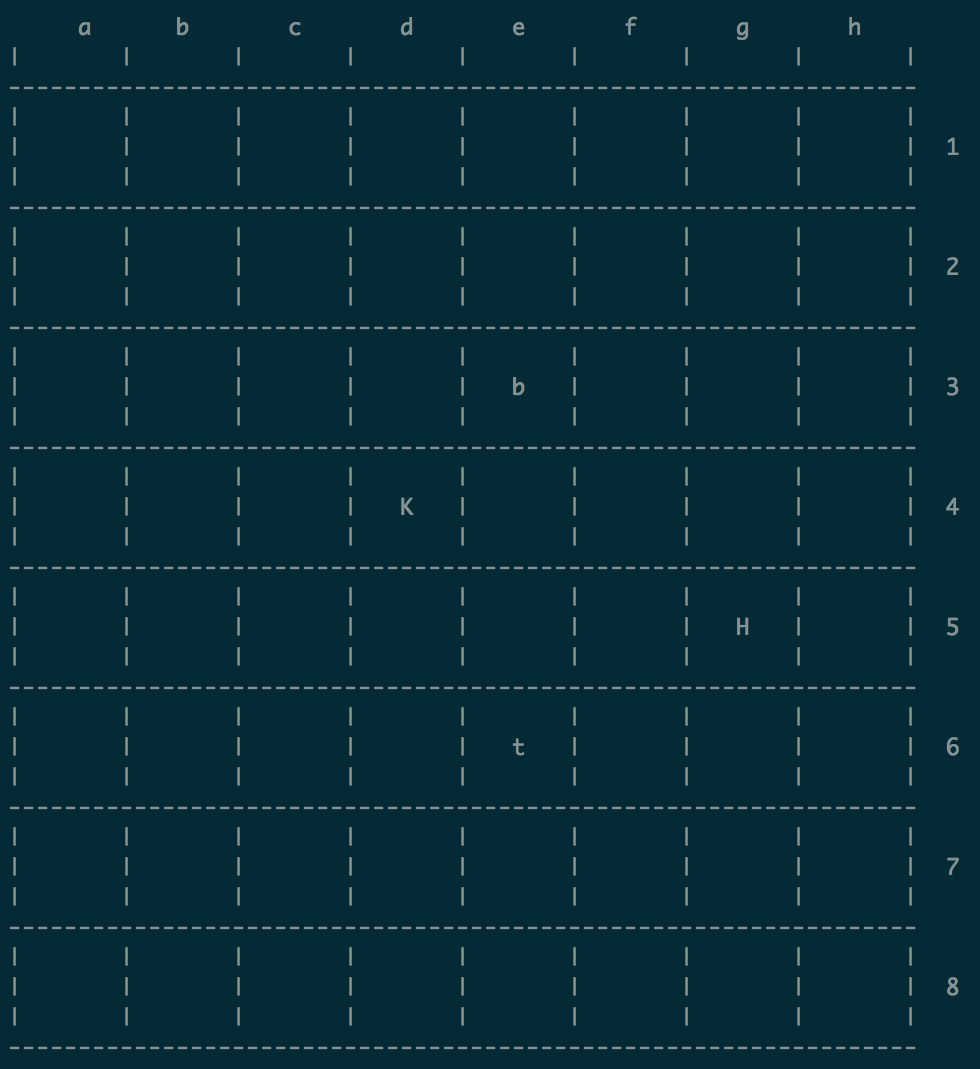
\includegraphics[scale=0.4]{board-texto-1.png}
\caption{\textit{ Representação textual do estado de jogo inicial.}}
\label{fig:fig5}
\endminipage\hfill
\minipage{0.3\textwidth}
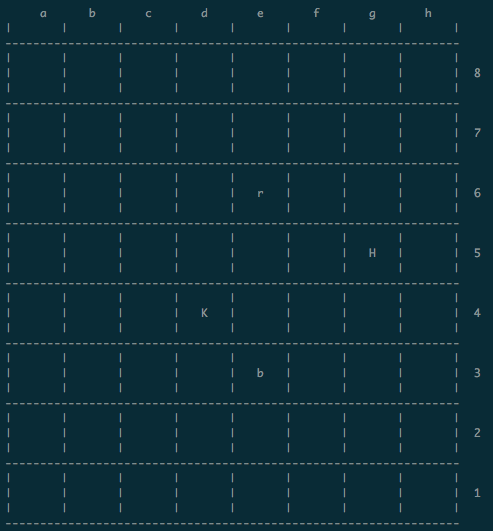
\includegraphics[scale=0.4]{board-texto-2.png}
\caption{\textit{ Representação textual de um estado intermédio.}}
\label{fig:fig6}
\endminipage
\end{figure}
\end{small}




%%%%%%%%%%%%%%%%%%%%%%%%%%
\section{Movimentos}

Como o jogo não permite alterar a posição de uma peça após a sua colocação no tabuleiro, nem é permitido captura das mesmas, apenas existe um tipo de movimentação.\linebreak

\Large Colocar uma peça no tabuleiro 
\begin{lstlisting}[language=Prolog]
setPiece( Piece, Row, Column, Board).
\end{lstlisting}

\end{document}
